\documentclass[a4paper]{article}
\usepackage[12pt]{extsizes} 
\usepackage[utf8]{inputenc}
\usepackage[russian]{babel}
\usepackage{setspace,amsmath,amssymb, fontenc, enumitem, multicol, caption, wrapfig, tikz, lipsum}
\usepackage{graphicx}
\usepackage[left=30mm, top=15mm, right=20mm, bottom=15mm, nohead, footskip=10mm]{geometry}
\usetikzlibrary{angles, quotes}

\definecolor{ochre}{RGB}{204,119,34}

\begin{document} 
	% НАЧАЛО ТИТУЛЬНОГО ЛИСТА
	\begin{center}
		\footnotesize{ФЕДЕРАЛЬНОЕ ГОСУДАРСТВЕННОЕ АВТОНОМНОЕ БЮДЖЕТНОЕ ОБРАЗОВАТЕЛЬНОЕ}\\ 
		\footnotesize{УЧРЕЖДЕНИЕ ВЫСШЕГО ОБРАЗОВАНИЯ}\\
		\small{\textbf{«НАЦИОНАЛЬНЫЙ ИССЛЕДОВАТЕЛЬСКИЙ УНИВЕРСИТЕТ ИТМО»}}\\[10pt]
		\normalsize{(ФПИиКТ)}\\[220pt]
		\large{Лабораторная №6}\\
		\large{Работа с системой компьютерной вёрстки TeX}\\
		\large{Вариант 49}\\[180pt]
	\end{center}
	
	\begin{flushright}
		Выполнил: \\
		Студент группы Р3115 \\
		Зыков Иван Евгеньевич \\[14pt]
		Проверил:\\
		Авксентьева Елена Юрьевна, \\
		к.п.н., доцент факультета ПИиКТ\\[80pt]
	\end{flushright}
	
	\begin{center} 
		Санкт-Петербург 2023 
	\end{center}
	\thispagestyle{empty} 
	% КОНЕЦ ТИТУЛЬНОГО ЛИСТА
	%\raggedright
	\newpage
	\tableofcontents
	
	\newpage
	\section{Задание}
	\subsection{Подготовка к работе}
		\begin{enumerate}[label=\arabic*.]
			\item Скачать и установить любой дистрибутив TEX (например, MiKTeX) или создать
			аккаунт на сайте ShareLaTeX (sharelatex.com), Overleaf (overleaf.com) или
			любом аналогичном.
			\item Выбрать год и номер журнала «Квант» (kvant.ras.ru) согласно варианту из
			таблицы на последней странице документа. Вариант выбирается как сумма
			после\-днего числа в номере группы, умноженного на 10, и номера в списке
			группы согласно ISU на текущий день.
			\item Выбрать одну страницу из всего номера, отвечающую следующим требованиям:
			\begin{itemize}
				\item Текст должен состоять минимум из 2 колонок.
				\item Заголовок не должен превышать 20% от площади страницы.
				\item Страница должна содержать 1 или 2 картинки, общая площадь которых
				не должна превышать 40% площади страницы.
				\item Текст должен содержать не менее 2 сложных формул. Желательно, чтобы
				были такие математические операции, как сумма элементов (не путать с
				простым сложением), извлечение корня, логарифм и т.п.
				\item В тексте должна быть как минимум 1 таблица. Размерность таблицы
				должна превышать 2*2 элемента.
			\end{itemize}
			В случае, если такая страница не найдена, то взять 1.5 страницы, где на одной
			будет большая часть задания, а на оставшейся – меньшая.
			В случае, если и таким образом страница не найдена, необходимо увеличить
			год выпуска на 19 лет и искать материал в новом выпуске.
		\end{enumerate}
	\subsection{Обязательное задание}
		Сверстать страницу, максимально похожую на выбранную страницу из журнала
		«Квант».
	\subsection{Дополнительное задание №1}
		\begin{enumerate}[label=\arabic*.]
			\item Сверстать титульный лист.
			\item Создать файл main.tex, в котором будет содержаться преамбула и ссылки на 2
			документа: титульный лист и статью (ссылки создаются с помощью команды
			input).
		\end{enumerate}
	\subsection{Дополнительное задание №2}
		Выполнение данного задания позволяет получить до 15 дополнительных
		процентов от максимального числа баллов БаРС за данную лабораторную.
		\begin{enumerate}[label=\arabic*.]
			\item Рассчитать номер варианта по следующей схеме:\\
			\textit{Ф – количество букв в фамилии, И – количество букв в имени}\\
			\textit{Номер варианта = 1 + ((Ф * И) mod 27)}
			\item Выполнить задание из полученного варианта, используя средства LaTeX.\\
			1) Сформировать таблицу периодических элементов
			Д.И.
			Менделеева,
			максимально похожую на предложенную:
			2-16) Используя pdf-документ (книга «ПЕРВЫЕ ШЕСТЬ КНИГ НАЧАЛ
			ЕВКЛИДА») сверстать 1 страницу. При этом геометрические фигуры и
			отрезки должны быть нарисованы, а не вставлены как картинка. Можно
			использовать любой удобный для вас способ рисования.
			\begin{itemize}
				\item2 – стр. 26
				\item3 – стр. 28
				\item4 – стр. 29
				\item5 – стр. 31
				\item6 – стр. 37
				\item7 – стр. 40
				\item8 – стр. 46
				\item9 – стр. 48
				\item10 – стр. 49
				\item11 – стр. 50
				\item12 – стр. 51
				\item13 – стр. 59
				\item14 – стр. 74
				\item15 – стр. 89
				\item16 – стр. 96
			\end{itemize}
			17-27) Используя пакет MusiXTeX написать не менее 25 первых нот гимна страны,
			название которой на русском языке начинается со следующей буквы:
			\begin{itemize}
				\item17 – А
				\item18 – Б
				\item19 – В
				\item20 – Г
				\item21 – Д
				\item22 – З
				\item23 – К
				\item24 – Л
				\item25 – М
				\item26 – Н
				\item27 – Р
			\end{itemize}
		\end{enumerate}
	\newpage
	\section{Выполнение}
		\subsection{Обязательное задание}
		\begin{figure}[h]
			\centering
			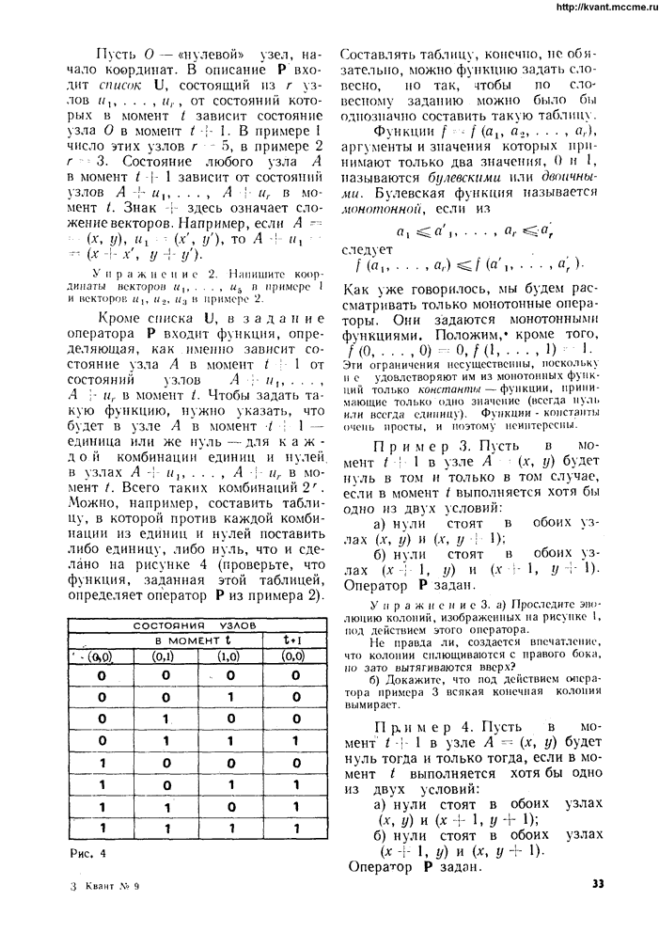
\includegraphics[width=0.85\textwidth]{Kvant.png}
			\caption{страница из журнала квант}
			\label{fig:квант}
		\end{figure}
	\newpage
	\begin{multicols}{2}
		Пусть $O$ - "нулевой" \ узел, начало координат. В описание $\textbf{P}$ входит \textit{список} $\textbf{U}$, состоящий из $r$ узлов $u_1, ... , u_r$, от состояний которых в момент $t$ зависит состояние узла $O$ в момент $t+1$. В примере 1 число этих узлов $r-5$, в примере 2 \ $r - 3$. Состояние любого узла $A$ в момент $t+1$ зависит от состояний узлов $A + u_1, ... , A + u_r$ в момент $t$. Знак + здесь означает сложение векторов. Например, если $A = (x, y), \ u_1 = (x', y')$, то $A + u_1 = (x + x', y + y')$.\\[10pt]
		\small{\textit{У п р а ж н е н и е 2.} Напишите координаты векторов $u_1, ... , u_5$ в примере 1 и векторов $u_1, u_2, u_3$ в примере 2.}\\[10pt]
		Кроме списка \textbf{U}, в \textit{з а д а н и е} оператора \textbf{P} входит функция, определяющая, как именно зависит состояние узла $A$ в момент $t + 1$ от состояния узлов $A + u_1, ... , A + u_r$ в момент $t$. Чтобы задать такую функцию, нужно указать, что будет в узле $A$ в момент $t + 1$ - единица или же нуль - для к а ж д о й  комбинации единиц и нулей в узлах $A + u_1, ... , A + u_r$ в момент $t$. Всего таких комбинаций $2^r$. Можно, например, составить таблицу, в которой против каждой комбинации из единиц и нулей поставить либо единицу, либо нуль, что и сделано на рисунке 4 (проверьте, что функция, заданная этой таблицей, определяет оператор \textbf{P} из примера 2).\\ 
		\begin{minipage}{\linewidth}
			\centering
			\begin{tabular}{|c|c|c|c|}
				\hline
				\multicolumn{4}{|c|}{Состояние узлов}\\
				\hline
				\multicolumn{3}{|c|}{в момент $t$} & $t + 1$\\ 
				\hline
				$(0,0)$ & $(0,1)$ & $(1,0)$ & $(0,0)$ \\
				\hline
				0 & 0 & 0 & 0 \\
				\hline
				0 & 0 & 1 & 0 \\
				\hline
				0 & 1 & 0 & 0 \\
				\hline
				0 & 1 & 1 & 1 \\
				\hline
				1 & 0 & 0 & 0 \\
				\hline
				1 & 0 & 1 & 1 \\
				\hline
				1 & 1 & 0 & 1 \\
				\hline
				1 & 1 & 1 & 1 \\
				\hline
			\end{tabular}
		\end{minipage}
		Составлять таблицу, конечно, не обязательно, можно функцию задать словесно, но так, чтобы по слоесному заданию можно было бы однозначно составить такую таблицу.\\
		Функции $f = f(a_1, a_2,..., a_r)$, аргументы и значения которых принимают только два значения, 0 и 1, называются \textit{булевскими} или \textit{двоичными}. Булевская функция называется \textit{монотонной}, если из 
		\begin{center}
			$ a_1 \leq a'_1, ..., a_r \leq a'_r$
		\end{center}
		следует 
		\begin{center}
			$ f(a_1, ..., a_r) \leq f(a'_1, ..., a'_r)$.
		\end{center}
		Как уже говорилось, мы будем рассматривать только монотонные операторы. Они задаются \textit{монотонными} функциями. Положим, кроме того, $f(0,..., 0) = 0$, $f (1,..., 1) = 1$.\\
		\small{Эти ограничения несущественны, поскольку удовлетворяют им из монотонных функций только \textit{константы} — функции, принимающие только одно значение (всегда нуль или всегда единицу). Функции константы очень просты, и поэтому неинтересны.}\\
		П р и м е р 3. Пусть в момент $t + 1$ в узле $A + (x, y)$ будет нуль в том и только в том случае, если в момент $t$ выполняется хотя бы одно из двух условий:
		\begin{enumerate}
			\item нули стоят в обоих узлах $(x, y)$ и\\ $(x, y + 1)$;
			\item нули стоят обоих узлах $(x + 1, y)$ и $(x + 1, y + 1)$. Оператор \textbf{Р} задан.
		\end{enumerate}
		\small{Упражнение 3. а) Проследите эволюцию колоний, изображенных на рисунке 1, под действием этого оператора.}\\
		\small{Не правда ли, создается впечатление, что колонии сплющиваются с правого бока, но зато \textit{вытягиваются} вверх?}\\
		\small{б) Докажите, что под действием опера- тора примера 3 всякая конечная вымирает.}\\
		П р и м е р 4. Пусть момент $t+1$ в узле $А = (x, y)$ будет нуль тогда и только тогда, если в момент $t$ выполняется хотя бы одно из двух условий:
		а) нули стоят в обоих узлах $(x, y)$ и $(x + 1, y + 1)$;
		б) нули стоят в обоих узлах $(x + 1, y)$ и $(x, y + 1)$. Оператор Р задан.
	\end{multicols}
	
	\newpage
	\subsection{Дополнительное задание №2}
		Вариант 10\\
		\begin{figure}[h]
			\centering
			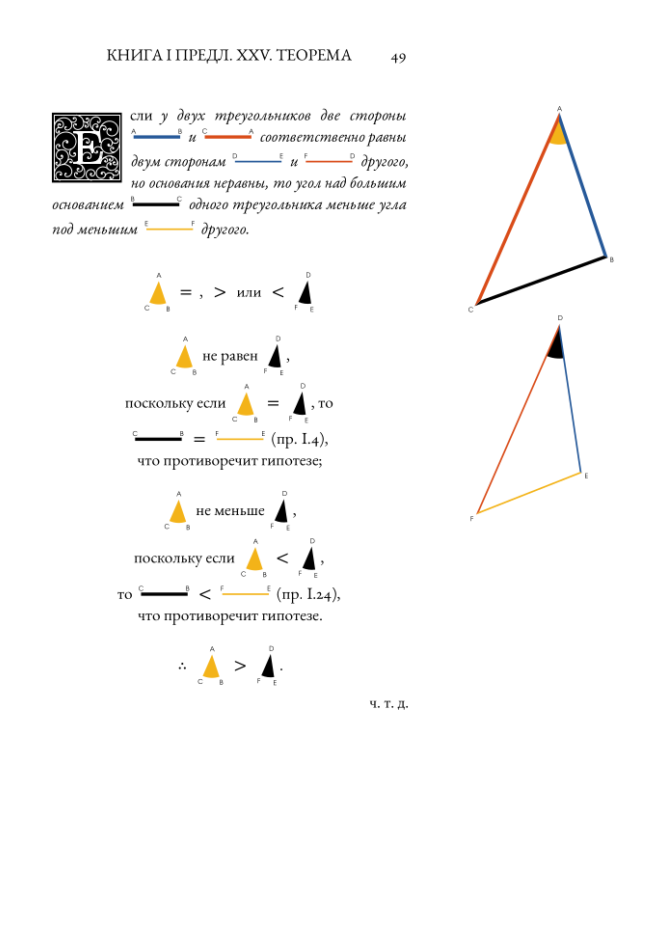
\includegraphics[width=0.9\textwidth]{dop2.png}
			\caption{страница из книги}
			\label{fig:dop2}
		\end{figure}
		
		\newpage
		\newgeometry{left=30mm, top=15mm, right=-25mm, bottom=15mm, nohead, footskip=10mm}
		\large{КНИГА I ПРЕД. XXV. ТЕОРЕМА}\\
		\begin{multicols}{2}
			\begin{wrapfigure}[5]{l}{0\textwidth}
				
\includegraphics[width=0.15\textwidth]{буква Е.png}
			\end{wrapfigure}
			\noindent \textit{сли у двух треугольников две стороны}
			\begin{tikzpicture}
				% Определение координат вершин треугольника
				\coordinate (A) at (0,0);
				\coordinate (B) at (1.5,0);
				
				% Рисование треугольника с разноцветными сторонами
				\draw[blue, line width=1mm] (A) -- (B);
				
				% Подписи вершин
				\node[above, font=\small] at (A) {$A$};
				\node[above, font=\small] at (B) {$B$};
			\end{tikzpicture}
			\textit{и}
			\begin{tikzpicture}
				% Определение координат вершин треугольника
				\coordinate (A) at (0,0);
				\coordinate (C) at (1.5,0);
				
				% Рисование треугольника с разноцветными сторонами
				\draw[red, line width=1mm] (C) -- (A);
				
				% Подписи вершин
				\node[above, font=\small] at (A) {$A$};
				\node[above, font=\small] at (C) {$C$};
			\end{tikzpicture} 
			\textit{соответственно равны двум сторонам}
			\begin{tikzpicture}
				% Определение координат вершин треугольника
				\coordinate (D) at (0,0);
				\coordinate (E) at (1.5,0);
				
				% Рисование треугольника с разноцветными сторонами
				\draw[blue, line width=0.5mm] (D) -- (E);
				
				% Подписи вершин
				\node[above, font=\small] at (D) {$D$};
				\node[above, font=\small] at (E) {$E$};
			\end{tikzpicture}
			\textit{и}
			\begin{tikzpicture}
				% Определение координат вершин треугольника
				\coordinate (F) at (0,0);
				\coordinate (D) at (1.5,0);
				
				% Рисование треугольника с разноцветными сторонами
				\draw[red, line width=0.5mm] (F) -- (D);
				
				% Подписи вершин
				\node[above, font=\small] at (F) {$F$};
				\node[above, font=\small] at (D) {$D$};
			\end{tikzpicture} 
			\textit{другого, но основания неравны, то угол над большим основанием}
			\begin{tikzpicture}
				% Определение координат вершин треугольника
				\coordinate (B) at (0,0);		
				\coordinate (C) at (1.5,0);
				
				% Рисование треугольника с разноцветными сторонами
				\draw[black, line width=1mm] (B) -- (C);
				
				% Подписи вершин
				\node[above, font=\small] at (B) {$B$};
				\node[above, font=\small] at (C) {$C$};
			\end{tikzpicture}
			\textit{обного треугольника меньше угла над меньшим}
			\begin{tikzpicture}
				% Определение координат вершин треугольника
				\coordinate (E) at (0,0);
				\coordinate (F) at (1.5,0);
				
				% Рисование треугольника с разноцветными сторонами
				\draw[orange, line width=0.5mm] (E) -- (F);
				
				% Подписи вершин
				\node[above, font=\small] at (E) {$E$};
				\node[above, font=\small] at (F) {$F$};
			\end{tikzpicture} 
			\textit{другого.}\\
			\begin{center}
				\begin{tikzpicture}
					\coordinate (A) at (0,1);
					\coordinate (B) at (-0.25,0);			
					\coordinate (C) at (0.25,0);
					
					\fill[orange] (A) -- (B) -- (C) -- cycle;
					
					\pic [draw, angle radius=1cm, orange, line width=1mm] {angle = B--A--C};
					\node[above, font=\tiny] at (A) {$A$};
					\node[below, font=\tiny] at (B) {$B$};
					\node[below, font=\tiny] at (C) {$C$};
					
					\node[anchor=west] at (0.7,0.1) {=, > или < };
				\end{tikzpicture}
				\begin{tikzpicture}
					\coordinate (D) at (0,1);
					\coordinate (F) at (-0.25,0);
					\coordinate (E) at (0.25,0);
					
					\fill[black] (D) -- (F) -- (E) -- cycle;
					
					\pic [draw, angle radius=1cm, black, line width=1mm] {angle = F--D--E};
					\node[above, font=\tiny] at (D) {$D$};
					\node[below, font=\tiny] at (F) {$F$};
					\node[below, font=\tiny] at (E) {$E$};
					
					
				\end{tikzpicture}\\
				
				\begin{tikzpicture}
					\coordinate (A) at (0,1);
					\coordinate (B) at (-0.25,0);
					\coordinate (C) at (0.25,0);
					
					\fill[orange] (A) -- (B) -- (C) -- cycle;
					
					\pic [draw, angle radius=1cm, orange, line width=1mm] {angle = B--A--C};
					\node[above, font=\tiny] at (A) {$A$};
					\node[below, font=\tiny] at (B) {$B$};
					\node[below, font=\tiny] at (C) {$C$};
					
					\node[anchor=west] at (0.7,0.1) {не равен};
				\end{tikzpicture}
				\begin{tikzpicture}
					\coordinate (D) at (0,1);
					\coordinate (F) at (-0.25,0);
					\coordinate (E) at (0.25,0);
					
					\fill[black] (D) -- (F) -- (E) -- cycle;
					
					\pic [draw, angle radius=1cm, black, line width=1mm] {angle = F--D--E};
					\node[above, font=\tiny] at (D) {$D$};
					\node[below, font=\tiny] at (F) {$F$};
					\node[below, font=\tiny] at (E) {$E$};
					
					\node[anchor=west] at (0.2,0.1) {,};
				\end{tikzpicture}\\
				
				\begin{tikzpicture}
					\coordinate (A) at (0,1);
					\coordinate (B) at (-0.25,0);
					\coordinate (C) at (0.25,0);
					
					\fill[orange] (A) -- (B) -- (C) -- cycle;
					
					\pic [draw, angle radius=1cm, orange, line width=1mm] {angle = B--A--C};
					\node[above, font=\tiny] at (A) {$A$};
					\node[below, font=\tiny] at (B) {$B$};
					\node[below, font=\tiny] at (C) {$C$};
					
					\node[anchor=east] at (-0.7,0.1) {поскольку если};
					\node[anchor=west] at (0.7,0.1) {=};
				\end{tikzpicture}
				\begin{tikzpicture}
					\coordinate (D) at (0,1);
					\coordinate (F) at (-0.25,0);
					\coordinate (E) at (0.25,0);
					
					\fill[black] (D) -- (F) -- (E) -- cycle;
					
					\pic [draw, angle radius=1cm, black, line width=1mm] {angle = F--D--E};
					\node[above, font=\tiny] at (D) {$D$};
					\node[below, font=\tiny] at (F) {$F$};
					\node[below, font=\tiny] at (E) {$E$};
					
					\node[anchor=west] at (0.2,0) {, то};
				\end{tikzpicture}\\
				
				
				\begin{tikzpicture}
					% Определение координат вершин треугольника
					\coordinate (B) at (0,0);
					\coordinate (C) at (1.5,0);
					
					% Рисование треугольника с разноцветными сторонами
					\draw[black, line width=1mm] (B) -- (C);
					
					% Подписи вершин
					\node[above, font=\small] at (B) {$B$};
					\node[above, font=\small] at (C) {$C$};
				\end{tikzpicture}
				=
				\begin{tikzpicture}
					% Определение координат вершин треугольника
					\coordinate (E) at (0,0);
					\coordinate (F) at (1.5,0);
					
					% Рисование треугольника с разноцветными сторонами
					\draw[orange, line width=0.5mm] (E) -- (F);
					
					% Подписи вершин
					\node[above, font=\small] at (E) {$E$};
					\node[above, font=\small] at (F) {$F$};
				\end{tikzpicture} 
				(пр. 1.4),\\
				что противоречит гипотезе\\
				
				\begin{tikzpicture}
					\coordinate (A) at (0,1);
					\coordinate (B) at (-0.25,0);
					\coordinate (C) at (0.25,0);
					
					\fill[orange] (A) -- (B) -- (C) -- cycle;
					
					\pic [draw, angle radius=1cm, orange, line width=1mm] {angle = B--A--C};
					\node[above, font=\tiny] at (A) {$A$};
					\node[below, font=\tiny] at (B) {$B$};
					\node[below, font=\tiny] at (C) {$C$};
					
					\node[anchor=west] at (0.7,0.1) {не меньше};
				\end{tikzpicture}
				\begin{tikzpicture}
					\coordinate (D) at (0,1);
					\coordinate (F) at (-0.25,0);
					\coordinate (E) at (0.25,0);
					
					\fill[black] (D) -- (F) -- (E) -- cycle;
					
					\pic [draw, angle radius=1cm, black, line width=1mm] {angle = F--D--E};
					\node[above, font=\tiny] at (D) {$D$};
					\node[below, font=\tiny] at (F) {$F$};
					\node[below, font=\tiny] at (E) {$E$};
					
					\node[anchor=west] at (0.2,0.1) {,};
				\end{tikzpicture}\\
				
				\begin{tikzpicture}
					\coordinate (A) at (0,1);
					\coordinate (B) at (-0.25,0);
					\coordinate (C) at (0.25,0);
					
					\fill[orange] (A) -- (B) -- (C) -- cycle;
					
					\pic [draw, angle radius=1cm, orange, line width=1mm] {angle = B--A--C};
					\node[above, font=\tiny] at (A) {$A$};
					\node[below, font=\tiny] at (B) {$B$};
					\node[below, font=\tiny] at (C) {$C$};
					
					\node[anchor=east] at (-0.7,0.1) {поскольку если};
					\node[anchor=west] at (0.7,0.1) {<};
				\end{tikzpicture}
				\begin{tikzpicture}
					\coordinate (D) at (0,1);
					\coordinate (F) at (-0.25,0);
					\coordinate (E) at (0.25,0);
					
					\fill[black] (D) -- (F) -- (E) -- cycle;
					
					\pic [draw, angle radius=1cm, black, line width=1mm] {angle = F--D--E};
					\node[above, font=\tiny] at (D) {$D$};
					\node[below, font=\tiny] at (F) {$F$};
					\node[below, font=\tiny] at (E) {$E$};
					
					\node[anchor=west] at (0.2,0.1) {,};
				\end{tikzpicture}\\
				
				то
				\begin{tikzpicture}
					% Определение координат вершин треугольника
					\coordinate (B) at (0,0);
					\coordinate (C) at (1.5,0);
					
					% Рисование треугольника с разноцветными сторонами
					\draw[black, line width=1mm] (B) -- (C);
					
					% Подписи вершин
					\node[above, font=\small] at (B) {$B$};
					\node[above, font=\small] at (C) {$C$};
				\end{tikzpicture}
				<
				\begin{tikzpicture}
					% Определение координат вершин треугольника
					\coordinate (E) at (0,0);
					\coordinate (F) at (1.5,0);
					
					% Рисование треугольника с разноцветными сторонами
					\draw[orange, line width=0.5mm] (E) -- (F);
					
					% Подписи вершин
					\node[above, font=\small] at (E) {$E$};
					\node[above, font=\small] at (F) {$F$};
				\end{tikzpicture} 
				(пр. 1.24),\\
				что противоречит гипотезе.\\
				
				\begin{tikzpicture}
					\coordinate (A) at (0,1);
					\coordinate (B) at (-0.25,0);
					\coordinate (C) at (0.25,0);
					
					\fill[orange] (A) -- (B) -- (C) -- cycle;
					
					\pic [draw, angle radius=1cm, orange, line width=1mm] {angle = B--A--C};
					\node[above, font=\tiny] at (A) {$A$};
					\node[below, font=\tiny] at (B) {$B$};
					\node[below, font=\tiny] at (C) {$C$};
					
					\node[anchor=west] at (0.7,0.1) {>};
				\end{tikzpicture}
				\begin{tikzpicture}
					\coordinate (D) at (0,1);
					\coordinate (F) at (-0.25,0);
					\coordinate (E) at (0.25,0);
					
					\fill[black] (D) -- (F) -- (E) -- cycle;
					
					\pic [draw, angle radius=1cm, black, line width=1mm] {angle = F--D--E};
					\node[above, font=\tiny] at (D) {$D$};
					\node[below, font=\tiny] at (F) {$F$};
					\node[below, font=\tiny] at (E) {$E$};
					
					\node[anchor=west] at (0.2,0.1) {.};
				\end{tikzpicture}\\
				
			\end{center}

			\columnbreak
			\begin{tikzpicture}
				% Определение координат вершин треугольника
				\coordinate (A) at (16,10);
				\coordinate (B) at (17,5);
				\coordinate (C) at (13,4);
				
				% Рисование треугольника с разноцветными сторонами
				\draw[blue, line width=1mm] (A) -- (B);
				\draw[black, line width=1mm] (B) -- (C);
				\draw[red, line width=1mm] (C) -- (A);
				
				\pic [draw, angle radius=1cm, orange, line width=1mm, fill] {angle = C--A--B};

				% Подписи вершин
				\node[above] at (A) {$A$};
				\node[below] at (B) {$B$};
				\node[below] at (C) {$C$};
			\end{tikzpicture}\\
			\begin{tikzpicture}
				% Определение координат вершин треугольника
				\coordinate (D) at (16,10);
				\coordinate (F) at (16.7,4.8);
				\coordinate (E) at (14,3.8);
				
				% Рисование треугольника с разноцветными сторонами
				\draw[blue, line width=1mm] (D) -- (F);
				\draw[orange, line width=1mm] (F) -- (E);
				\draw[red, line width=1mm] (E) -- (D);
				
				\pic [draw, angle radius=1cm, black, line width=1mm, fill] {angle = E--D--F};
				
				% Подписи вершин
				\node[above] at (D) {$D$};
				\node[below] at (F) {$F$};
				\node[below] at (E) {$E$};
			\end{tikzpicture}
		\end{multicols}
		\restoregeometry
		\newpage
\end{document}